\chapter{Rigidity: An Introduction} 

\begin{flushleft}
Rigidity can be easily understood as observing a structure and questioning how 'stiff' it is. If some force is applied to it, does it bend or buckle? When we pull the structure across (Euclidean) space, do we move it entirely, or does a part of it bend and move in the direction of the pull? As stiffness can be interpreted in a multitude of ways, this chapter will be dedicated to formalizing the definition of rigidity that we will use for the remainder of this project. 
\end{flushleft}

\begin{flushleft}
To start, we must first understand what a \textit{graph} is.
\end{flushleft}

\section{Graph Theory}

\begin{flushleft}
Here, we delve into a small portion of a very large field of mathematics. The definitions presented here will be fundamental for what's to come. This section is mostly adapted from Sophie Huczynska's lecture notes on Graph Theory \cite{graph_theory}.
\end{flushleft}

\begin{definition}
A \textit{graph} $G = (V,E)$ consists of a set V and a set E of two-element subsets of V. The elements of V are called \textit{vertices} (or nodes) and the elements of E are called \textit{edges}.
\end{definition}

\begin{example}
The graph $G = (V,E)$ below has $|V| = 5$, and $|E| = 5$.
\label{eg: cycle}
\begin{figure}[ht]
    \centering
    \documentclass{standalone}
\usepackage{tikz}
\usetikzlibrary{arrows,backgrounds,positioning,petri, calc}


\begin{document}
% Set the style for the vertices
\tikzstyle{vertex} = [circle, draw=black, fill = black, thin, inner sep=0pt,minimum size=2mm]

\begin{tikzpicture}
    
    % Define nodes
    \node (1) at (0,0) [vertex, label=left:$1$] {};
    \node (2) at (1,1) [vertex, label=above:$2$] {};
    \node (3) at (2.5,1) [vertex, label=above:$3$] {};
    \node (4) at (2.5,-1) [vertex, label=below:$4$] {};
    \node (5) at (1,-1) [vertex, label=below:$5$] {};

    % add edges
    \path[] (1) edge (2)
                edge (5)
            (3) edge (2)
                edge (4)
            (4) edge (5);
    
\end{tikzpicture}
\end{document}

% when entering figures, use the following format

%\begin{figure}[htbp]
%    \centering
%    \input{Chapter 1/framework}
%    \caption{Caption}
%    \label{fig:enter-label}
%\end{figure}
\end{figure}
\end{example}

\begin{definition} 
\begin{enumerate}
    \item A \textit{walk} in a graph $G$ is a sequence of vertices $u_1, \hdots, u_n$ such that $u_iu_{i+1}$ is an edge of $G$ for all $1 \leq i \leq n-1$.
    \item A walk whose vertices are all distinct is called a \textit{path}.
    \item A \textit{closed walk} is a walk $u_1, \hdots, u_n$ in $G$ such that $u_1 = u_n$.
    \item The \textit{length} of a walk or a path is the number of edges in it.
\end{enumerate}
\end{definition}

\begin{example}
Consider the graph in Example \ref{eg: cycle}. A path from vertex 1 to vertex 3 can either follow 123, or 1543.
\end{example}

\begin{definition}
A graph $G$ is \textit{connected} if for any two distinct vertices $u,v \in V(G)$, there exists a path between them.
\end{definition}

\begin{definition}
The \textit{degree} of a vertex is the number of edges incident to the vertex.
\end{definition}

\begin{flushleft}
There are several ways of drawing the 'same' graph on the plane. This includes labelling them in a variety of ways as well. Therefore, it is vital that we class these drawings as the same graph.
\end{flushleft}

\begin{definition}
\label{def: isomorphism}
Two graphs $G_1$ and $G_2$ are said to be \textit{isomorphic} if there is a bijection $\phi$ : $V(G_1) \rightarrow V(G_2)$ such that $xy \in E(G_1)$ if and only if $\phi(x)\phi(y) \in E(G_2)$. The function $\phi$ is known as an \textit{isomorphism}.
\end{definition}

\begin{example}
\label{eg: isomorphic graphs}
Consider the two graphs below.

\begin{figure}[ht]
    \centering
    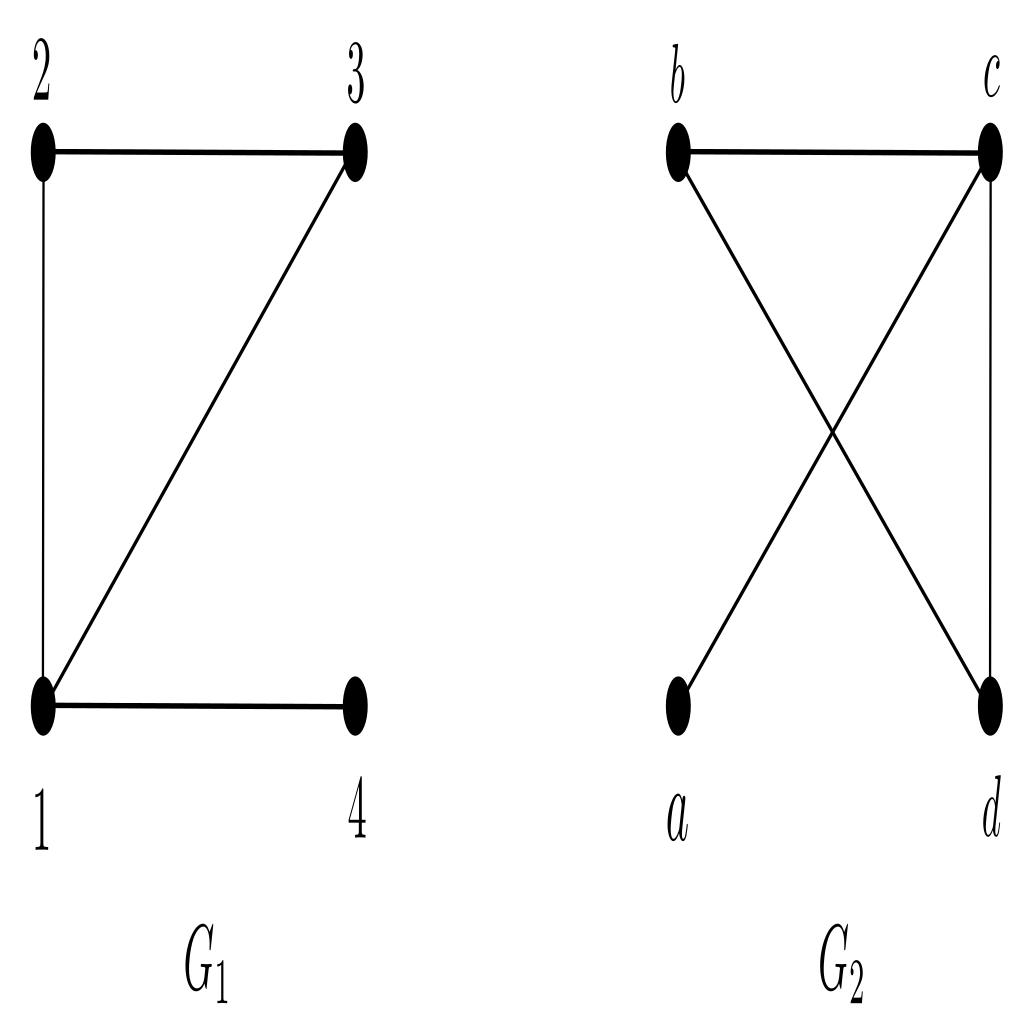
\includegraphics[width = 0.5\textwidth]{Chapter 2/3. isomorphic graphs .png}
    %\caption{Caption}
    \label{fig:isomoprhic graphs}
\end{figure}
\vspace{-5 mm}
\begin{flushleft}
The bijection $\phi : G_1 \rightarrow G_2$ is given by $\phi(1) = c$, $\phi(2) = b$, $\phi(3) = c$, and $\phi(4) = a$.    
\end{flushleft}
\end{example}

\begin{flushleft}
Given a graph $G$, we may be interested in a certain subset of vertices and edges that are included in $G$. This involves studying a \textit{subgraph} of $G$.
\end{flushleft}

\begin{definition}
A graph $H$ is a \textit{subgraph} of $G$ if there is a graph $H'$ isomorphic to $H$ such that $V(H') \subseteq V(G)$ and $E(H') \subseteq E(G)$.
\end{definition}

\begin{flushleft}
A subgraph $H$ can be obtained from a graph $G$ by a sequence of vertex and edge removals.
\end{flushleft}

\begin{example}
Consider the graphs below.

\begin{figure}[ht]
    \centering
    \documentclass{standalone}
\usepackage{tikz}
\usetikzlibrary{arrows,backgrounds,positioning,petri, calc}


\begin{document}
% Set the style for the vertices
\tikzstyle{vertex} = [circle, draw=black, fill = black, thin, inner sep=0pt,minimum size=2mm]

\begin{tikzpicture}
    
    % Define nodes
    \node (1) at (0,0) [vertex, label=left:$1$] {};
    \node (2) at (1,1) [vertex, label=above:$2$] {};
    \node (3) at (3,1) [vertex, label=above:$3$] {};
    \node (4) at (3,-1) [vertex, label=below:$4$] {};
    \node (5) at (1,-1) [vertex, label=below:$5$] {};
    \node[draw = none] (G1) at (2,-2.25) [label=above:$G$] {};

    \node (21) at (6,0) [vertex, label=left:$1$] {};
    \node (22) at (7,1) [vertex, label=above:$2$] {};
    \node (25) at (7,-1) [vertex, label=below:$5$] {};
    \node[draw = none] (H) at (7,-2.25) [label=above:$H$] {};
    

    % add edges
    \path[] (1) edge (2)
                edge (5)
            (3) edge (2)
                edge (4)
            (4) edge (5)
            (2) edge (5)
            (21) edge (22)
                edge (25)
            (22) edge (25);
    
\end{tikzpicture}
\end{document}

    %\caption{Caption}
    %\label{fig:enter-label}
\end{figure}
\noindent
If we remove the vertices 3 and 4, and all the edges incident to these two vertices from the graph $G$, we obtain the graph $H$, where $H$ is a subgraph of $G$.
\end{example}

\begin{flushleft}
The graphs we are interested in for this project are those such that the edges do not cross over each other. Such graphs are known to be \textit{planar}.
\end{flushleft}

\begin{definition}
    \label{def: planar graphs}
    A graph $G$ is \textit{planar} if it has a drawing in the plane such that none of edges cross over each other. Such a drawing $D$ is called a \textit{planar} drawing of $G$.
\end{definition}

\begin{example}
    Consider \hyperref[eg: isomorphic graphs]{Example \ref*{eg: isomorphic graphs}}. The graphs $G_1$ and $G_2$ are isomorphic, so they can be viewed as the `same' graph $G$. However, the drawing on the left is a planar drawing of $G$, whereas the drawing on the right is a non-planar drawing.
\end{example}

\begin{flushleft}
The last idea we need from graph theory is the notion of a \textit{face} of a planar graph. 
\end{flushleft}

\begin{definition}
Let $G$ be a planar graph, and let $D$ be a planar drawing of $G$. Then A \textit{face} of $D$ is a maximal section of the plane in which any two points can be joined by a curve which does not intersect any part of $D$. 
\end{definition}

\noindent
We can think of the faces as the regions into which the edges of D divide the plane. This idea becomes particularly useful when investigating the isomorphism of graphs obtained through computational means later on.

\begin{definition}
Let $G$ be a planar graph, and let $D$ be a planar drawing of $G$. The \textit{length} of a face of $D$ is the total length of the closed walk in $D$ that bounds it.
\end{definition}

\noindent
That is, when we trace round the boundary of a face in D, we traverse a
sequence of vertices and edges, before returning to our start point. The number of edges traversed in this sequence is the length of the face.

\section{Frameworks}

\begin{flushleft}
Now that we have a good idea of what graphs are, we can start working on setting up frameworks. The definitions in this section will be defined in the space $\mathbb{R}^d$, where $d \in \mathbb{N}$. Later, we will find ourselves working exclusively in $\mathbb{R}^2$. For the remainder of this chapter, we shall adhere closely to the contents in the book ``Frameworks, Tensegrities, and Symmetry'' by Robert Connelly and Simon D. Guest \cite{textbook}.
\end{flushleft}

\noindent
The first definition we need is that of a \textit{configuration}.

\begin{definition}
    Suppose we have a collection of $n$ labelled points in $\mathbb{R}^d$, where $d \in \mathbb{N}$. Let $\mathbf{p}_i = (p_{i1}, \hdots, p_{id})$ be the position vector of point $i$. Then a \textit{configuration} is

\[
\mathbf{p} = (\mathbf{p}_1, \hdots, \mathbf{p}_n),
\]

\begin{flushleft}
where $\mathbf{p}$ is a vector of vectors in $\mathbb{R}^d$.     
\end{flushleft}
\end{definition}

\begin{flushleft}
Therefore, a configuration is a set of points in the space $\mathbb{R}^d$, each point equipped with its own position vector. Henceforth, we will refer the the points in a configuration as \textit{nodes}. 
\end{flushleft}

\begin{flushleft}
Given a configuration $\mathbf{p}$, we can now decide which pairs of nodes to connect with a graph $G$. The nodes in $\mathbf{p}$ correspond to the vertices in $G$, and $G$ is not allowed to have multiple edges between vertices, or loops between the same vertex (such graphs are known to be \textit{simple}).
\end{flushleft}

\begin{definition}
    A \textit{framework} is a configuration $\mathbf{p} = (\mathbf{p}_1, \hdots, \mathbf{p}_n)$ together with its corresponding graph $G = (V,E)$. We denote a framework as $(G,\mathbf{p})$.
\end{definition}

\begin{flushleft}
Note that as we are working in $\mathbb{R}^d$, the \textit{length} of each edge with endpoints $\mathbf{p}_i$ and $\mathbf{p}_j$ in a framework $(G,\mathbf{p})$ is the \textit{Euclidean distance} between the nodes $\mathbf{p}_i$ and $\mathbf{p}_j$. This is denoted $|\mathbf{p}_i - \mathbf{p}_j|$.

In this project, graphs will be drawn with vertices that are filled in, whereas frameworks will have hollow nodes. 
\end{flushleft}

%\clearpage

\begin{example}
\label{g vs f}
Consider Figure \ref{fig: graph vs framework}. The drawing on the left is a graph, whereas the drawing on the right is a framework.
    \begin{figure}[htbp]
        \centering
        \documentclass{standalone}
\usepackage{tikz}
\usetikzlibrary{arrows,backgrounds,positioning,petri, calc}


\begin{document}
% Set the style for the vertices
\tikzstyle{vertex} = [circle, draw=black, thin, inner sep=0pt,minimum size=2mm]

\begin{tikzpicture}
    
    % Define nodes for the first K4
    \node (11) at (0,0) [vertex, fill = black] {};
    \node (12) at (0,2) [vertex, fill = black] {};
    \node (13) at (2,2) [vertex, fill = black] {};
    \node (14) at (2,0) [vertex, fill = black] {};

    % add invisible node at (1,-1)
    \node[draw = none] (graph) at (1, -.5) {Graph};

    % define nodes for the second K4
    \node (21) at (4,0) [vertex] {};
    \node (22) at (4,2) [vertex] {};
    \node (23) at (6,2) [vertex] {};
    \node (24) at (6,0) [vertex] {};

    \node[draw = none] (graph) at (5, -.5) {Framework};

    % add the edges
    \path[] (11) edge (12)
                edge (14)
            (12) edge (13)
            (13) edge (11)
                edge (14); 

    \path[] (21) edge (22)
                edge (24)
            (22) edge (23)
            (23) edge (21)
                edge (24); 
\end{tikzpicture}
\end{document}
        \caption{}
        \label{fig: graph vs framework}
    \end{figure}
\end{example}

\begin{flushleft}
At this stage, you may be wondering what exactly the difference between a graph and a framework is. Put simply;
\begin{itemize}
    \item A graph is an abstract mathematical object that can be visualised in a multitude of ways, as seen in \hyperref[eg: isomorphic graphs]{Example \ref*{eg: isomorphic graphs}}. Varying the edge lengths does not produce a new graph as by \hyperref[def: isomorphism]{Definition \ref*{def: isomorphism}}, they are isomorphic, and considered the `same'.
    \vspace{-3mm}
    \item In a framework however, each node has a position vector. If we consider a framework in $\mathbb{R}^2$ such as the one in \hyperref[g vs f]{Figure \ref{fig: graph vs framework}}, each node is at a determined distance from each other. Slightly changing the position of a node results in a different framework.

\end{itemize}
\end{flushleft}

\begin{flushleft}
Frameworks are essential when it comes to studying the rigidity of structures. Considering real-world applications, a simple model of a building can be designed by considering what its framework would look like in $\mathbb{R}^3$. Investigating this framework allows for insight into how the building in question should be constructed.
\end{flushleft}

\noindent
Armed with the notion of a framework, we can begin thinking about how we might be able to change the shape of a framework. 

\section{Motions}

\begin{flushleft}
When it comes to studying the rigidity of frameworks, we begin by understanding what it means for a framework to experience a \textit{motion} (also known as a \textit{flex}). 
\end{flushleft}

\begin{definition}
Suppose the configuration $\mathbf{p} = (\mathbf{p}_1, \hdots, \mathbf{p}_n)$ is on a differentiable smooth path parameterized by time $t$, denoted $\mathbf{p}(t)$. Then 

    \begin{itemize}
        \item The position of node $\mathbf{p}_i \in \mathbf{p}$ at any time $t$ is given by $\mathbf{p}_i(t) \in \mathbb{R}^d$.
        \vspace{-3mm}
        \item The \textit{initial position} of a node $\mathbf{p}_i$ is $\mathbf{p}_i(0) \in \mathbb{R}^d$
        \vspace{-3mm}
        \item The \textit{initial configuration} of $\mathbf{p}$ is 
        \[
        \mathbf{p}(0) = (\mathbf{p}_1(0), \hdots, \mathbf{p}_n(0)) \in \mathbb{R}^{nd}
        \]
    \end{itemize}
\end{definition}

\begin{definition}
A \textit{motion} of the framework $(G,\mathbf{p})$ is a differentiable smooth path $\mathbf{p}(t)$ parameterized by time $t$ such that 

\[
|\mathbf{p}_i(t) - \mathbf{p}_j(t)| = |\mathbf{p}_i(0) - \mathbf{p}_j(0)|,
\]

\noindent
for all $t$, and for all $ij \in E(G)$.
\end{definition}

\begin{flushleft}
In other words, a motion preserves the length of every edge in the framework at any point in time. A motion $\mathbf{p}(t) = (\mathbf{p}_1(t), \hdots, \mathbf{p}_n(t))$ is a \textit{continuous motion} if each of the $d$ coordinates of $\mathbf{p}_i(t)$ are continuous in $t$. This means that the nodes must vary smoothly with time, without any abrupt changes or breaks.
\end{flushleft}

\begin{flushleft}
There are certain motions that we can apply to a framework such that the distances between all the nodes are preserved as well. Such motions are known as \textit{rigid motions}.
\end{flushleft}

\begin{definition}
A \textit{rigid motion} of the framework $(G,\mathbf{p})$ is a differentiable smooth path $\mathbf{p}(t)$ parameterized by time $t$ such that 

\[
|\mathbf{p}_i(t) - \mathbf{p}_j(t)| = |\mathbf{p}_i(0) - \mathbf{p}_j(0)|,
\]

\noindent
for all $t$, and for all $i, j \in V(G)$
\end{definition}

\begin{flushleft}
Given this definition, let us contemplate the ways in which we can apply a rigid motion to a given framework $(G,\mathbf{p})$. There are two natural ways in which we can apply a motion such that it preserves the distances between every node;
\end{flushleft}

\begin{itemize}
    \item \textit{Translating} the entire framework across $\mathbb{R}^d$ preserves the distances between each node, and so it is a rigid motion.
    \vspace{-3mm}
    \item \textit{Rotating} the entire framework about a point also preserves the distances between each node. Thus, it is a rigid motion as well.
    
\end{itemize}

\begin{flushleft}
In fact, these are the only two rigid motions available in $\mathbb{R}^d$. 
\end{flushleft}

\begin{theorem}
\label{thm: rigid motion theorem}
\cite{textbook} Let $(G,\mathbf{p})$ be a framework. Then a motion of $(G,\mathbf{p})$ is a rigid motion if there exists a positive-definite orthogonal $d \times d$ matrix $\mathbf{Q}(t)$, where $\mathbf{Q}(0)$ is the identity matrix, and a vector $\mathbf{w}(t) \in \mathbb{R}^d$, where $\mathbf{w}(0)$ is the zero vector, such that the position of every node is given by 

\[
\mathbf{p}_i(t) = \mathbf{Q}(t)\mathbf{p}_i + \mathbf{w}(t)
\]

\noindent
for all $i = 1, \hdots, n$.
\end{theorem}

\begin{flushleft}
The matrix $\mathbf{Q}(t)$ represents a rotation of the node $\textbf{p}_i$, and the vector $\mathbf{v}(t)$ represents a translation of $\textbf{p}_i$. In other words, Theorem \ref{thm: rigid motion theorem} states that any rigid motion of a framework can be viewed as a motion of the framework with a component pertaining to rotation, and one pertaining to translation.
\end{flushleft}


\begin{example}
\label{eg: simple motion}
Consider a framework with three nodes, labelled $\textbf{p}_1, \textbf{p}_2, \textbf{p}_3$, and two edges, $\textbf{p}_1\textbf{p}_2$, and $\textbf{p}_2\textbf{p}_3$. Apply the motion 

\[ \textbf{p}_i(t) = 
\begin{cases}
    \cos(t) - \sin(t), & \text{if } i = 3 \\
    \textbf{p}_i(0), & \text{if } i = 1,2
\end{cases}
\]

\vspace{3 mm}
\noindent
to this framework. A diagram of what happens for times $t=0$, and $t=1$ is shown below
%\clearpage

    \begin{figure}[htbp]
        \centering
        \documentclass{standalone}
\usepackage{tikz}
\usetikzlibrary{arrows,backgrounds,positioning,petri, calc}

\begin{document}
% Set the style for the vertices
\tikzstyle{vertex} = [circle, draw=black, thin, inner sep=0pt,minimum size=2mm]

\begin{tikzpicture}

    % before the motion
    \node (11) at (0,0) [vertex, label=above:$\textbf{p}_1$] {};
    \node (12) at (2,0) [vertex, label=above:$\textbf{p}_2$] {};
    \node (13) at (2,-2) [vertex, label=below:$\textbf{p}_3$] {};

    \node[draw = none] (t1) at (-0.2, -1.5) {$t = 0$};
    %\draw[->] (2.5,-1) -- (4.5,-1);
    % after the motion
    \node (21) at (5,0) [vertex, label=above:$\textbf{p}_1$] {};
    \node (22) at (7,0) [vertex, label=above:$\textbf{p}_2$] {};
    \node (23) at (5.6, -1.4) [vertex, label = below: $\textbf{p}_3$] {};

    \node[draw = none] (t2) at (4.5, -1) {$t = 1$};

    % add the edges before the motion
    \path[] (11) edge (12);
    \path[] (12) edge (13); % Make this edge red
    
    % Swing node (13) along an arc towards node (11)
    \path[draw, ->, dashed] (13) edge [bend left = 40] (11); 

    % add the edges before the motion
    \path[] (21) edge (22);
    \path[] (22) edge (23); % Make this edge red
    
    % Swing node (13) along an arc towards node (11)
    \path[draw, ->, dashed] (23) edge [bend left = 20] (21); 

\end{tikzpicture}
\end{document}

        \caption{A framework where the edge $\textbf{p}_2\textbf{p}_3$ can swing about $\textbf{p}_2$.}
        \label{fig: simple motion}
    \end{figure}
\vspace{-5 mm}
\begin{flushleft}
As all the edge lengths are preserved, this is a motion. However, the distance between nodes $\textbf{p}_1$ and $\textbf{p}_3$ changes as $t$ changes. Therefore, this is not a rigid motion.    
\end{flushleft}
\end{example}

\begin{example}
Consider the matrix 

\[ \mathbf{Q} = 
\begin{pmatrix}
-1 & 0\\
0 & -1\\
\end{pmatrix}
\]

\begin{flushleft}
This results in a rotation of each node by 180$\degree$ about the origin $O$ in $\mathbb{R}^2$. Applying this to the framework in \hyperref[eg: simple motion]{Example \ref*{eg: simple motion}} at $t = 0$, we obtain

\begin{figure}[htbp]
    \centering
    \documentclass{standalone}
\usepackage{tikz}
\usepackage{gensymb}
\usetikzlibrary{arrows,backgrounds,positioning,petri, calc}

\begin{document}
% Set the style for the vertices
\tikzstyle{vertex} = [circle, draw=black, thin, inner sep=0pt,minimum size=2mm]

\begin{tikzpicture}[node distance = 2cm, auto, scale = 1]

    %\tikzstyle{every node}=[font=\small]

    % before the motion
    \node (11) at (-1,0) [vertex, label=above:$\textbf{p}_1$] {};
    \node (12) at (1,0) [vertex, label=above:$\textbf{p}_2$] {};
    \node (13) at (1,-2) [vertex, label=below:$\textbf{p}_3$] {};

    % add node for the origin
    \node (origin) at (0,-1) [vertex, fill = black, label=below:$O$] {};

    % add an invisble node
    \node[draw = none] (start) at (1.2, -1) {};

    % add an invisible node for the label
    \node[draw = none] (label) at (3.5, -1)[label=above:Multiply by $\mathbf{Q}$]{};

    % after the motion
    \node (21) at (8,-2) [vertex, label=below:$\textbf{p}_1$] {};
    \node (22) at (6,-2) [vertex, label=below:$\textbf{p}_2$] {};
    \node (23) at (6, 0) [vertex, label = above: $\textbf{p}_3$] {};

    % add node for the origin
    \node (origin2) at (7, -1) [vertex, label = above: $O$, fill = black] {};

    % add an invisble node
    \node[draw = none] (end) at (5.8, -1) {};

    % add the edges before the motion
    \path[] (11) edge (12);
    \path[] (12) edge (13); % Make this edge red
    
    % add the edges before the motion
    \path[] (21) edge (22);
    \path[] (22) edge (23);  

    % plot the line between the diagrams
    \draw[->] (start) -- (end);
    

\end{tikzpicture}
\end{document}

\end{figure}

As all the edge lengths, as well as the distances between each node are preserved, this is a rigid motion.    
\end{flushleft}
\end{example}

\section{Rigidity}
\begin{flushleft}
As we have seen, rigid motions maintain not only the lengths of every edge in a framework, but they also fix the distance between each node as well. At this stage, we can question what frameworks can only be subject to rigid motions. Is there a framework such that the only way to move it is if we move \textit{all} of it?

The answer is yes, and such frameworks are said to be \textit{rigid}.
\end{flushleft}

\begin{definition}
\label{def: rigid}
A framework $(G,\mathbf{p})$ is rigid if every continuous motion $\mathbf{p}(t) = (\mathbf{p}_1(t), \hdots, \mathbf{p}_n(t))$ is a rigid motion. 
If a framework is not rigid, it is said to be \textit{flexible}.
\end{definition}

\begin{example}
\label{eg: rigid graphs}    
The frameworks in Figure \ref{fig: rigid_graphs} are rigid. 

\vspace{3mm}
\begin{figure}[htbp]
    \centering
    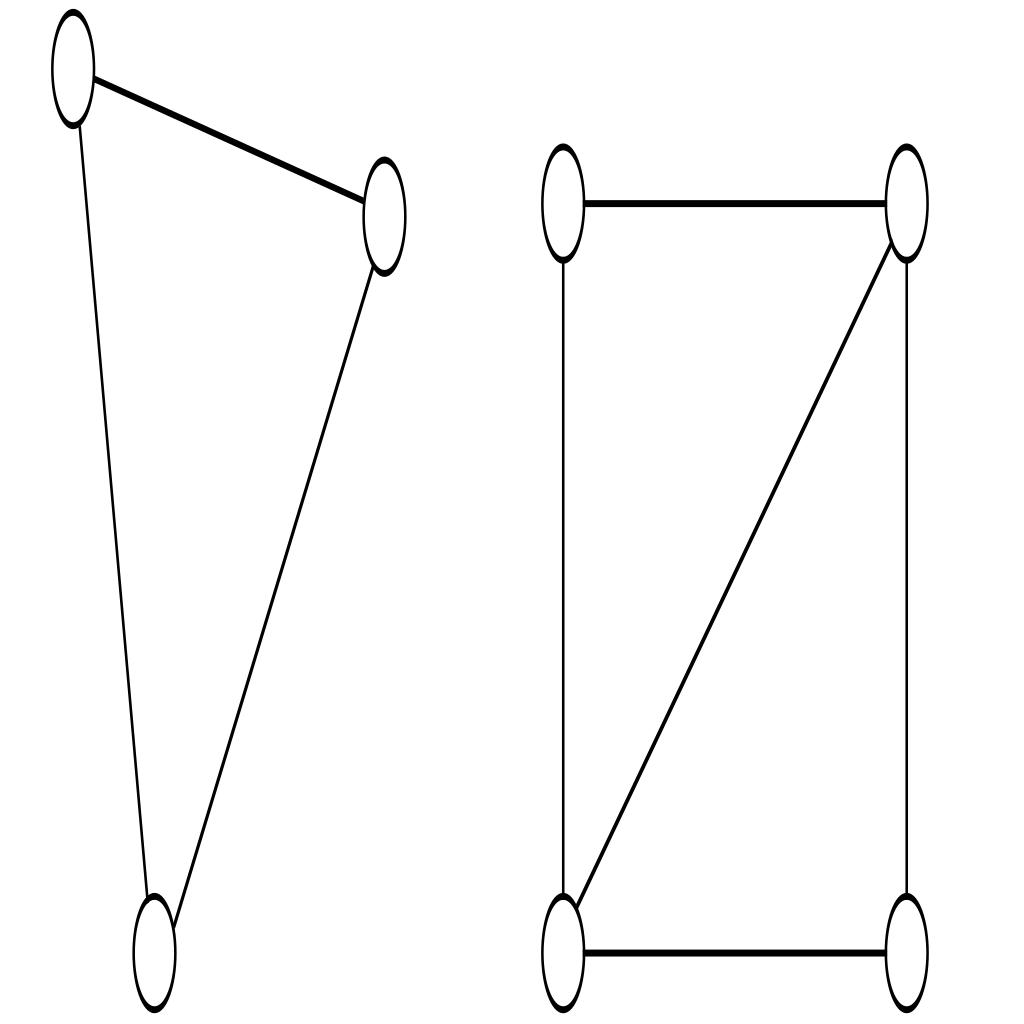
\includegraphics[width=0.57\textwidth]{Chapter 2/7. rigid_graphs.png} 
    \caption{Two rigid frameworks in $\mathbb{R}^2$}
    \label{fig: rigid_graphs}
\end{figure}
\vspace{-3mm}
\begin{flushleft}
However, the framework in Figure \ref{eg: not_rigid} is not. We can apply a motion to the nodes $\textbf{p}_1$ and $\textbf{p}_2$ such that the edge lengths are preserved, but the distance between the diagonal nodes change, violating the definition of rigidity.    
\end{flushleft}

\begin{figure}[htbp]
    \centering
    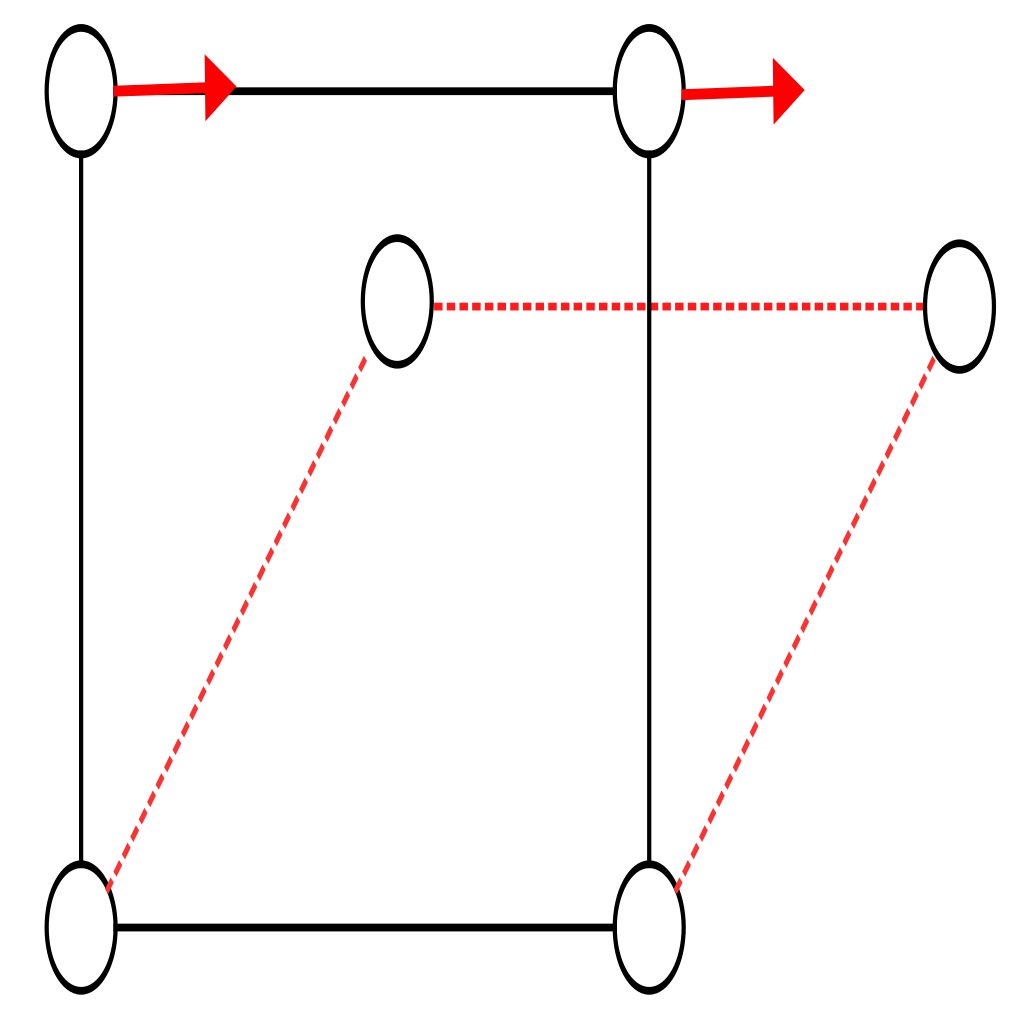
\includegraphics[width = 0.4\textwidth]{Chapter 2/8. not_rigid.png}
    \caption{A framework that is not rigid in $\mathbb{R}^2$}
    \label{eg: not_rigid}
\end{figure}
\end{example}
\vspace{-5 mm}
\begin{flushleft}

\vspace{-3mm}
Another equivalent definition of rigidity that was proved by Asimow and Roth \cite{asimow} uses ideas of the congruency of frameworks.
\end{flushleft}

\begin{definition}
Consider two frameworks $(G,\mathbf{p})$ and $(G,\mathbf{q})$ where $\mathbf{p} = (\mathbf{p}_1, \hdots, \mathbf{p}_n)$ and $\mathbf{q} = (\mathbf{q}_1, \hdots, \mathbf{q}_n)$.
\begin{itemize}
    \item $(G,\mathbf{q})$ is \textit{equivalent} to $(G,\mathbf{p})$ if $|\mathbf{p}_i - \mathbf{p}_j| = |\mathbf{q}_i - \mathbf{q}_j|$ for all $ij \in E(G)$.
    \vspace{-3mm}
    \item $(G,\mathbf{q})$ is \textit{congruent} to $(G,\mathbf{p})$ if $|\mathbf{p}_i - \mathbf{p}_j| = |\mathbf{q}_i - \mathbf{q}_j|$ for all $i, j \in V(G)$.
\end{itemize}
\end{definition}

\begin{flushleft}
In other words, two frameworks $(G,\mathbf{p})$ and $(G,\mathbf{q})$ are equivalent if the edge lengths are the same for every pair of labelled nodes in $(G,\mathbf{p})$. They are congruent if $(G,\mathbf{p})$ can be obtained through a series of rotations and translations of $(G,\mathbf{q})$. 
\end{flushleft}

% https://www.youtube.com/watch?v=kQlrqrjBXtk, 3:03
\begin{theorem}
\cite{asimow} A framework $(G,\mathbf{p})$ on $n$ nodes is \textit{rigid} if and only if there exists an $\epsilon > 0$ such that every framework $(G,\textbf{q})$ which is equivalent to $(G,\mathbf{p})$ and satisfies 

\[
|\mathbf{p}_i - \mathbf{q}_i| < \epsilon
\]
\begin{flushleft}
for all $i \in V(G)$, is congruent to $(G,\mathbf{p})$.  
\end{flushleft}
\end{theorem}

\begin{figure}[htbp]
    \centering
    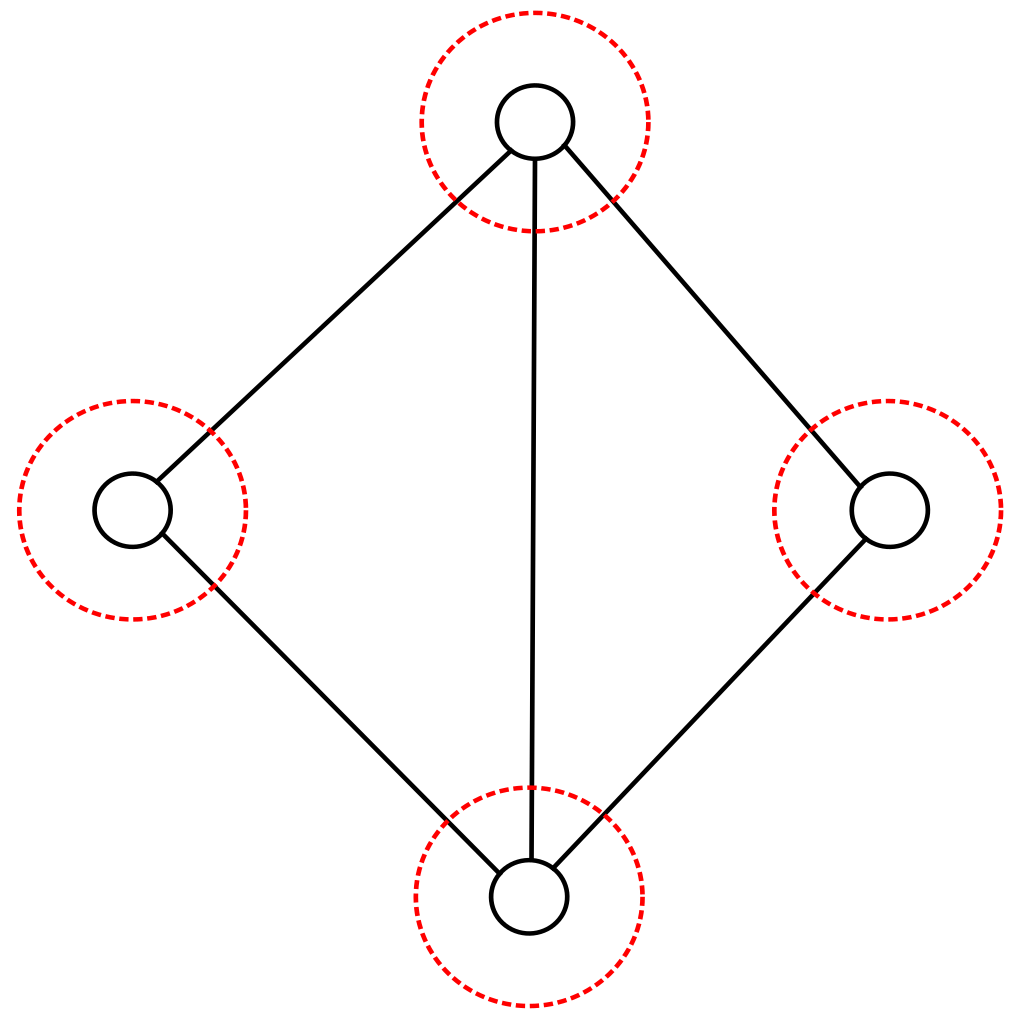
\includegraphics[width = 0.35\textwidth]{Chapter 2/14. epsilon.png}
    \caption{A framework $\mathbf{p}$ with an epsilon bound (red) for every node}
    \label{fig: epsilon}
\end{figure}
\vspace{-3mm}
\begin{flushleft}
In Figure \ref{fig: epsilon}, we visualise what an epsilon bound for every node for a framework $(G,\textbf{p})$ looks like. If we create a framework $(G,\textbf{q})$ such that it is equivalent to $(G,\mathbf{p})$, and the nodes of $(G,\mathbf{q})$ fall within the epsilon bounds of each corresponding node in $(G,\mathbf{p})$, then we are able to conclude that with some rigid motion, we are able to achieve congruence between $(G,\mathbf{p})$ and $(G,\mathbf{q})$. 

In such scenarios, equivalence implies congruence.    
\end{flushleft}

\subsection{Infinitesimal Rigidity}

\begin{flushleft}
In some sense, the definition of rigidity we have seems quite loose. Depending on the structure of a framework, a well placed `push' might be able to deform the framework, distorting the distances between the nodes in the framework.
\end{flushleft}

\begin{figure}[htbp]
    \centering
    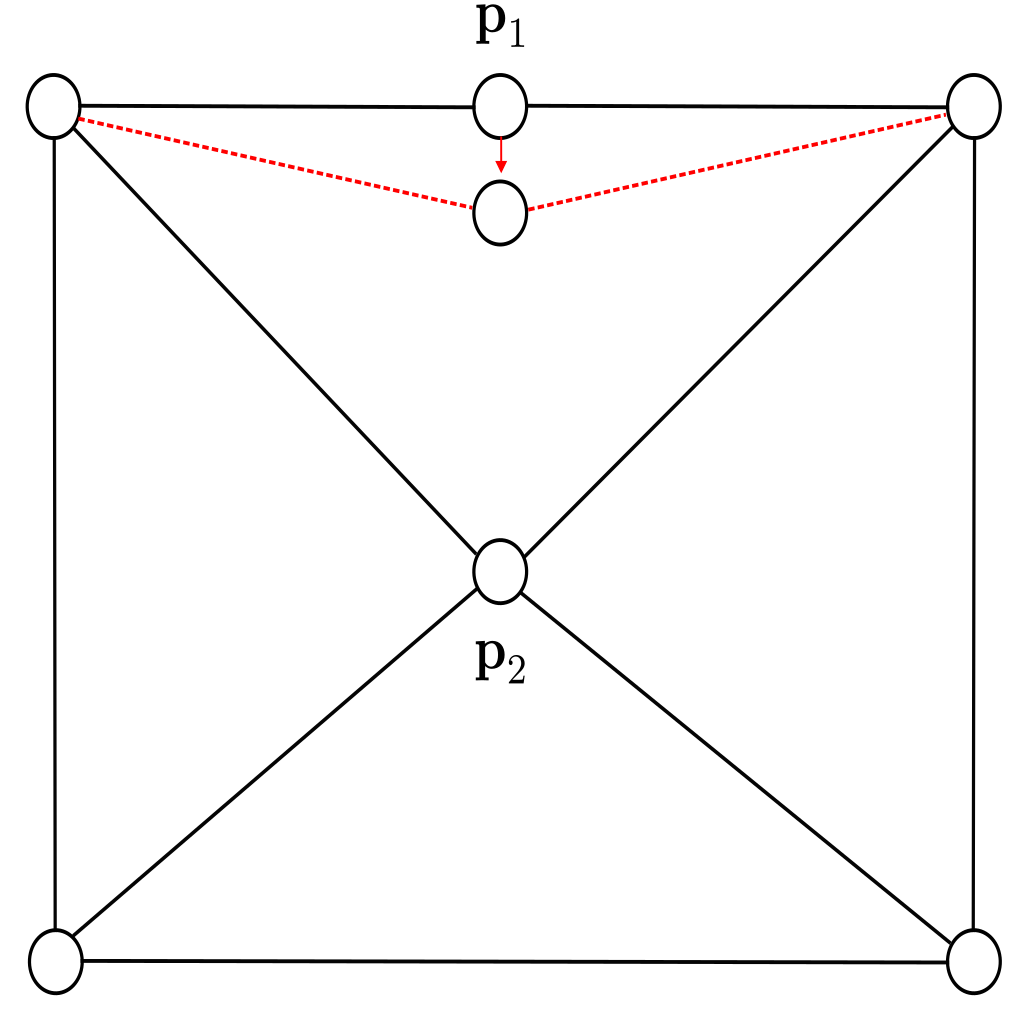
\includegraphics[width = 0.4\textwidth]{Chapter 2/9. not_inf_rigid.png}
    \caption{A framework where the node $\textbf{p}_1$ is `pushed' vertically down, deforming the framework. This is shown in red.}
    \label{fig: not_inf_rigid}
\end{figure}
\vspace{-3 mm}
\begin{flushleft}
Looking at the framework $(G,\textbf{p})$ in Figure \ref{fig: not_inf_rigid}, we can `push' the node $\textbf{p}_1$ vertically down. This act preserves all the edge lengths of $(G,\textbf{p})$, but the distance between $\textbf{p}_1$ and $\textbf{p}_2$ has now changed. Although the framework can be shown to be rigid (which we will see soon), it somehow doesn't `feel' rigid.
\end{flushleft}

\begin{flushleft}
In order to strengthen the definition of rigidity, let us first start with an observation described in greater detail by Graver in his book ``Counting on Frameworks'' \cite{counting_frameworks}. 
\end{flushleft}

\begin{flushleft}
Suppose that the configuration $\mathbf{p}$ is on a smooth differentiable path parameterized by time $t$. Consider a node of the configuration $\mathbf{p}_i$. Then its position is given by $\mathbf{p}_i(t)$ and as $\mathbf{p}_i$ is on a differentiable path, its derivative is well-defined.
\end{flushleft}

\begin{figure}[htbp]
    \centering
    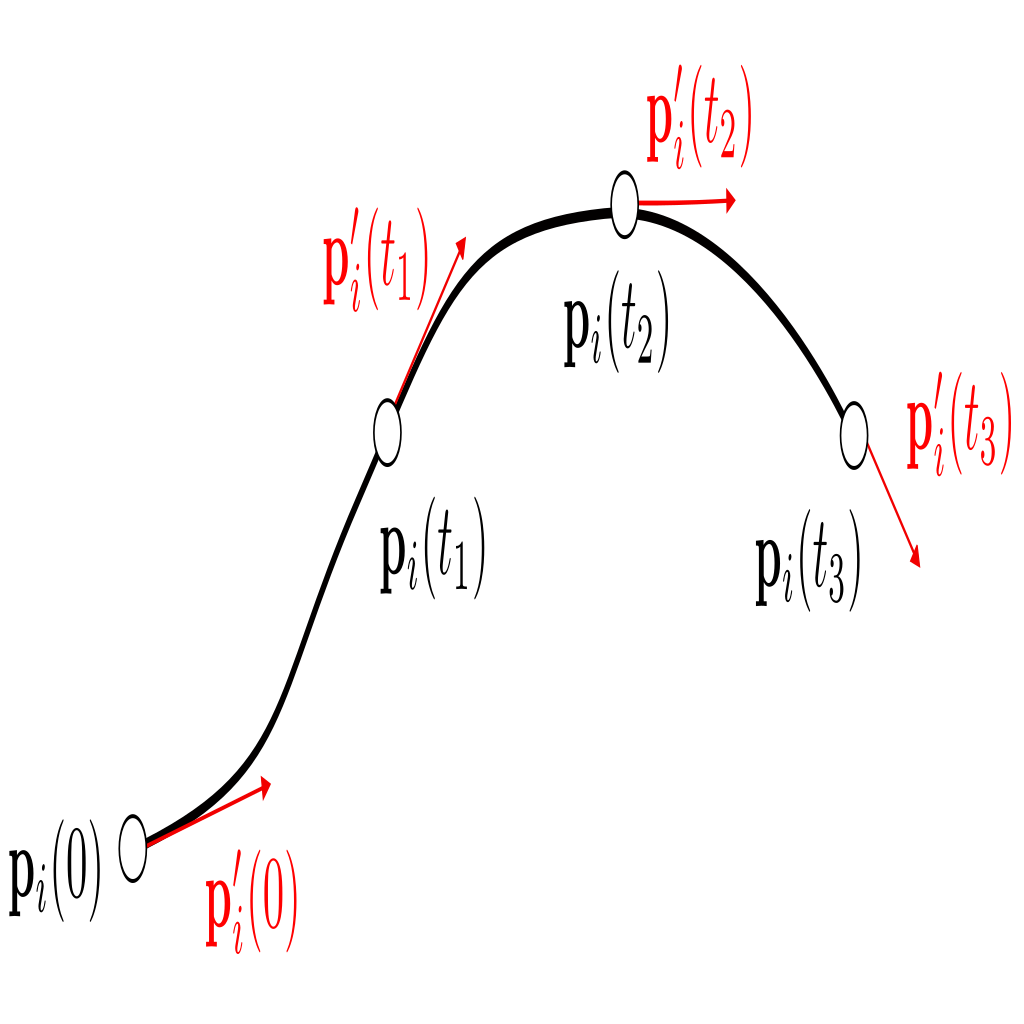
\includegraphics[width = 0.5\textwidth]{Chapter 2/12. path.png}
    \caption{Node $\mathbf{p}_i$ at various positions on path $\mathbf{p}_i(t)$ for various times $t$. The instantaneous velocities at each position $\mathbf{p}'_i(t)$ are marked in red}
    \label{fig: path}
\end{figure}

\vspace{-3mm}
\begin{definition}
    Let $(G,\mathbf{p})$ be a framework where each node is on a differentiable smooth path parameterized by $t$ such that the position of each node is given by $\mathbf{p}_i(t)$ for all $i \in  V(G)$. Then \textit{instantaneous velocity} of the node $\mathbf{p}_i(t)$ is given by
    
    \[
    \mathbf{p}'_i(t) = \frac{d\mathbf{p}_i(t)}{dt}
    \]
    
    \noindent
    for all $t$.
\end{definition} 

%\vspace{-5.5 mm}

\begin{flushleft}
The velocities $\mathbf{p}'_i(t)$ become vital when studying infinitesimal rigidity. To motivate this, let us consider a framework in $\mathbb{R}^2$.
\end{flushleft}

\begin{figure}[htbp]
    \centering
    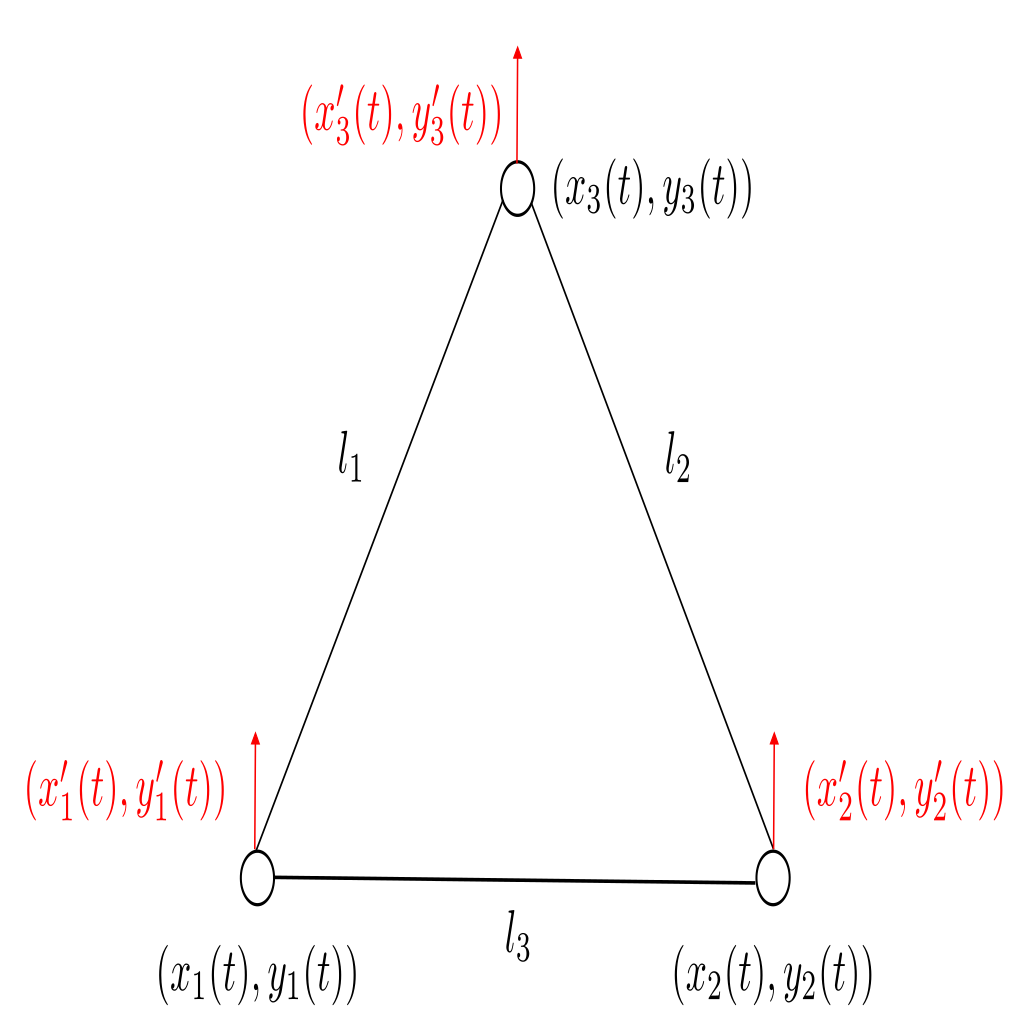
\includegraphics[width = 0.65\textwidth]{Chapter 2/13. inf_rigid_proof.png}
    \caption{A framework in $\mathbb{R}^2$, with some instantaneous velocity vectors at each node given in red.}
    \label{fig: inf_velocity}
\end{figure}

\vspace{-3mm}
\begin{flushleft}
In Figure \ref{fig: inf_velocity}, we have a framework with three nodes, each defined by coordinates $(x_i(t), y_i(t))$ as well as their corresponding velocities given by $(x'_i(t), y'_i(t))$ for $i = 1,2,3$. As each point is fixed in the plane, the distances between each pair of nodes are constants, given as $l_i$ for $i = 1,2,3$.
\end{flushleft}

\begin{flushleft}
Therefore, we know that 
%\vspace{-1 mm}
\[
\begin{split}
(x_1(t) - x_2(t))^2 + (y_1(t) - y_2(t))^2 = {l_3}^2 \\
(x_1(t) - x_3(t))^2 + (y_1(t) - y_3(t))^2 = {l_1}^2 \\
(x_2(t) - x_3(t))^2 + (y_2(t) - y_3(t))^2 = {l_2}^2
\end{split}
\]

Now, if we differentiate each equation with respect to $t$, we get 
%\vspace{-1 mm}
\[
\begin{split}
2(x_1 - x_2)(x'_1 - x'_2) + 2(y_1 - y_2)(y'_1 - y'_2) = 0 \\
2(x_1 - x_3)(x'_1 - x'_3) + 2(y_1 - y_3)(y'_1 - y'_3) = 0 \\
2(x_2 - x_3)(x'_2 - x'_3) + 2(y_2 - y_3)(y'_2 - y'_3) = 0
\end{split}
\]

where we drop the dependence on $t$ for notational convenience. By factoring out the $2$, these equations can be written as
%\vspace{-1 mm}
\[
\begin{split}
(x_1 - x_2, y_1 - y_2) \cdot (x'_1 - x'_2, y'_1 - y'_2) = 0 \\
(x_1 - x_3, y_1 - y_3) \cdot (x'_1 - x'_3, y'_1 - y'_3) = 0 \\
(x_2 - x_3, y_2 - y_3) \cdot (x'_2 - x'_3, y'_2 - y'_3) = 0
\end{split}
\]

Or more simply
%\vspace{-1 mm}
\[
(x_i - x_j, y_i - y_j) \cdot (x'_i - x'_j, y'_i - y'_j) = 0
\]

for all $i,j = 1,2,3$ where $i \neq j$.
\end{flushleft}

\begin{flushleft}
This observation allows us to impose conditions such that edge lengths and node distances are preserved when velocities are applied to a node, enabling us to study rigidity in even finer detail. With this in mind, let us formalize what we have just seen.
\end{flushleft}

\begin{flushleft}
The instantaneous velocity of a node allows us to consider what happens to a framework as we attempt to deform it by applying some motion or force to every node. If we want a framework to be rigid in the conventional sense, then we enforce a condition such that the distances between all the nodes of the framework are preserved when such velocities are applied to the nodes of the framework. 
\end{flushleft}

\begin{definition}
\label{def: inf motion}
Let $(G,\mathbf{p})$ be a framework where each node is on a differentiable smooth path parameterized by time $t$ such that the position of each node is given by $\mathbf{p}_i(t)$ for all $i \in  V(G)$. 
\begin{itemize}
    \item An \textit{infinitesimal motion} of $(G,\mathbf{p})$ is given by $(\mathbf{p}_i - \mathbf{p}_j) \cdot (\mathbf{p}'_i - \mathbf{p}'_j) = 0$ for all $ij \in  E(G)$. 
    \vspace{-3mm}
    \item An infinitesimal motion is an \textit{infinitesimal rigid motion} of $(G,\mathbf{p})$ if $(\mathbf{p}_i - \mathbf{p}_j) \cdot (\mathbf{p}'_i - \mathbf{p}'_j) = 0$ for all $i,j \in  V(G)$. 
\end{itemize}
\noindent
Therefore, we obtain a system of equations, where the $(\mathbf{p}'_i - \mathbf{p}'_j)$ terms are unknown, and $(\mathbf{p}_i - \mathbf{p}_j)$ terms form our coefficients. In Chapter 3, we will revisit this system of equations to uncover a theorem that allows us to determine whether a given framework is rigid or not.
\end{definition}

\begin{flushleft}
As we saw when considering Figure \ref{fig: inf_velocity}, an infinitesimal motion of a framework is the assignment of an instantaneous velocities $\mathbf{p}'_i$ to nodes $\mathbf{p}_i$ such that the length of the edge $|\mathbf{p}_i - \mathbf{p}_j|$ remains constant for all edges $ij \in E(G)$ to the first order. Analogously to before, if we can apply infinitesimal motions to the framework such that it preserves the distance between every node, then we have an infinitesimal rigid motion. 
\end{flushleft}

\begin{flushleft}
We have already seen that for a framework to be rigid in space, all of its motions must be rigid motions. A similar conclusion can be drawn here as well.
\end{flushleft}

\begin{definition}
\label{def: inf rigid}
Let $(G,\mathbf{p})$ be a framework where each node is on a differentiable smooth path parameterized by time $t$ such that the position of each node is given by $\mathbf{p}_i(t)$ for all $i \in  V(G)$. Then $(G,\mathbf{p})$ is \textit{infinitesimally rigid} if all of its infinitesimal motions are infinitesimal rigid motions.

\noindent
If a framework is not infinitesimally rigid, it is \textit{infinitesimally flexible}.
\end{definition}

% https://www.researchgate.net/figure/a-A-rigid-framework-which-is-not-infinitesimally-rigid-b-An-infinitesimally-flexible_fig5_220452659
\begin{example}
Let us look at a framework that is infinitesimally flexible.
%\vspace{2mm}
\begin{figure}[htbp]
    \centering
    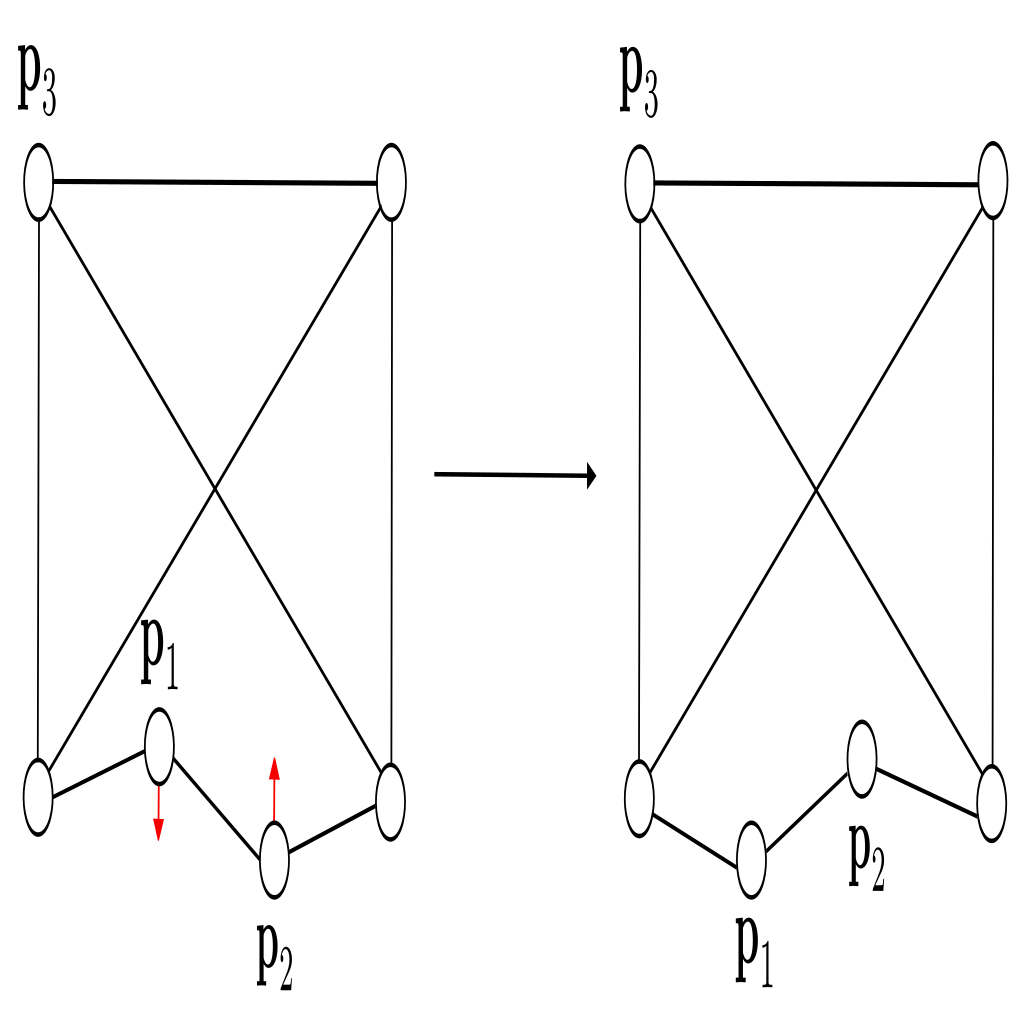
\includegraphics[width = 0.7\textwidth]{Chapter 2/10. not_inf_rigid_2.0.png}
    \caption{A framework that is not infinitesimally rigid}
    \label{eg: not inf rigid 2.0}
\end{figure}

\begin{flushleft}
By applying instantaneous velocities to nodes $\textbf{p}_1$ and $\textbf{p}_2$ as shown in the framework on the left of Figure \ref{eg: not inf rigid 2.0}, we restructure the framework such that all the edge lengths are kept constant. This is shown in the framework on the right. However, the distance between nodes $\textbf{p}_1$ and $\textbf{p}_3$ have been altered. Therefore, this framework is not infinitesimally rigid.
\end{flushleft}
     
\begin{figure}[htbp]
    \centering
    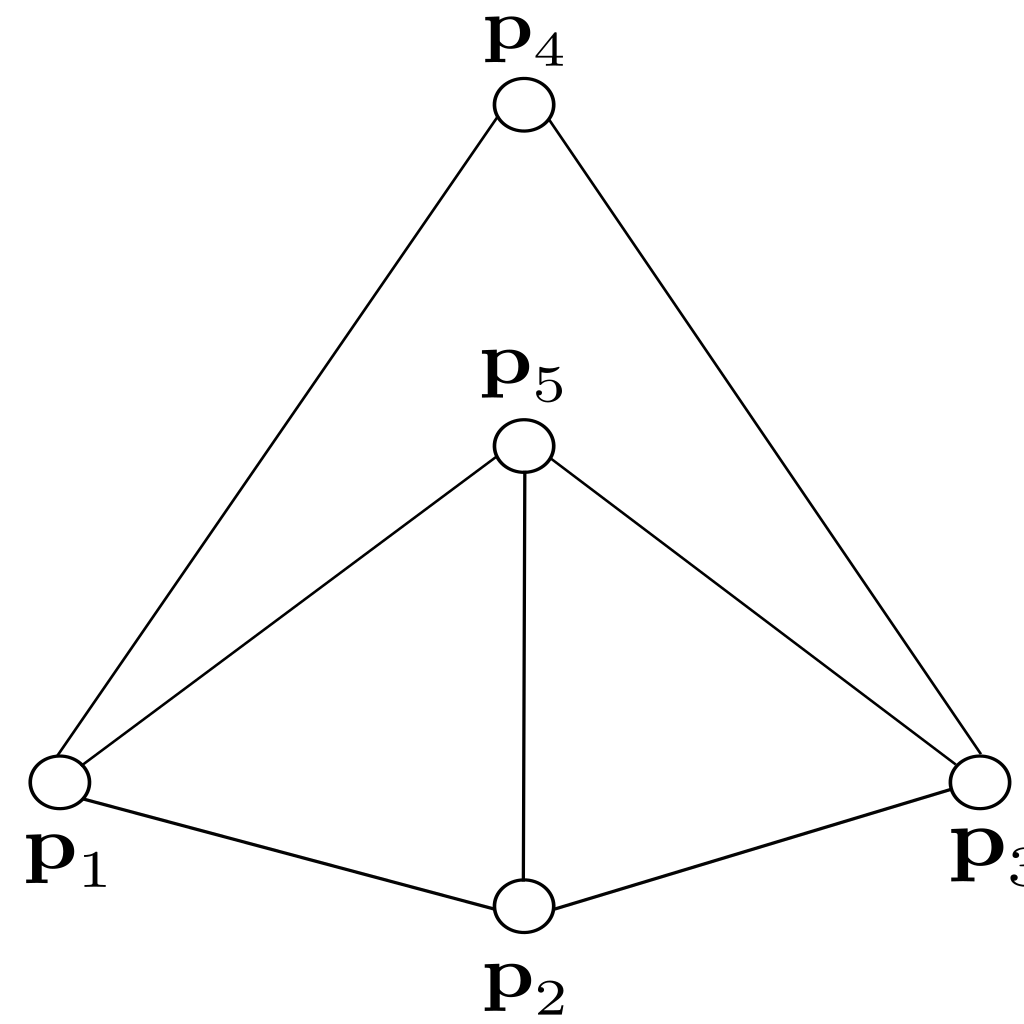
\includegraphics[width = 0.35\textwidth]{Chapter 2/11. inf_rigid.png}
    \caption{An infinitesimally rigid framework}
    \label{eg: inf rigid}
\end{figure}
\vspace{-2mm}
\begin{flushleft}
Now consider the framework in Figure \ref{eg: inf rigid}. As we will soon see, triangular frameworks are infinitesimally rigid by a process known as a Type I Henneberg construction \cite{henneberg}. So this means that the framework can not be deformed by applying instantaneous velocities to nodes $\textbf{p}_1,\textbf{p}_2,\textbf{p}_3$  or $\textbf{p}_5$.     
\end{flushleft}

\begin{flushleft}
As the only possible way we can deform this framework is by applying some velocity to $\textbf{p}_4$, let us apply a instantaneous velocity to displace $\textbf{p}_4$ by an infinitesimal distance, say to the left without loss of generality. As our edges are of a fixed length, this will require edge $\textbf{p}_3\textbf{p}_4$ to `pull' node $\textbf{p}_3$ upwards with the motion. As triangles $\textbf{p}_2\textbf{p}_3\textbf{p}_5$ and $\textbf{p}_1\textbf{p}_2\textbf{p}_5$ are known to be infinitesimally rigid, this causes the entire framework to rotate in an anti-clockwise fashion.
\end{flushleft}

\noindent
We already know that rotations are (infinitesimal) rigid motions, and so any displacement of the node $\textbf{p}_4$ results in an infinitesimal rigid motion. Therefore, we conclude that the framework in \hyperref[eg: inf rigid]{Figure 1.5} is infinitesimally rigid.
\end{example}

\subsection{Generic Rigidity}
We close this chapter on one last interesting way to classify rigidity. When studying configurations, we are interested in those that have nothing `special' about the way the nodes are arranged. Such configurations are known to be \textit{generic}.

\begin{flushleft}
To begin, we define a simpler phenomenon in order to get a feel for what we mean by not `special'.    
\end{flushleft}

\begin{definition}
\cite{discrete} Let $\mathbf{p} \in \mathbb{R}^d$ be a configuration. Then $\mathbf{p}$ is in \textit{general position} if any $d+1$ number of points do not lie in an $d-1$ dimensional affine subspace for $d>0$.
\end{definition}

\begin{flushleft}
Affine subspaces, and the mathematics involved in studying such structures can be found in texts relating to \textit{Discrete Geometry}, and it is beyond the scope of this project. The definition essentially says that for a set of points to be in general position, we must \textbf{not} have:
\begin{itemize}
    \item Any two points that coincide at the same point when $d = 1$.
    \vspace{-3mm}
    \item Any three points that lie on the same line when $d = 2$.
    \vspace{-3mm}
    \item Any four points that lie on the same plane when $d = 3$.
\end{itemize}

And the pattern continues. This gives us a set of points that are spread out, making them more interesting to study.
\end{flushleft}

\begin{flushleft} 
Genericity is a stronger condition than that of general position. The definition is as follows.
\end{flushleft}

\begin{definition}
A configuration $\mathbf{p}$ is \textit{generic} if the only polynomial with coefficients from $\mathbb{Q}$ that the coordinates of each point in $\mathbf{p}$ satisfies is the zero polynomial.
\end{definition}

\begin{example}
Figure \ref{fig: not generic points} displays two configurations.

    \begin{figure}[htbp]
        \centering
        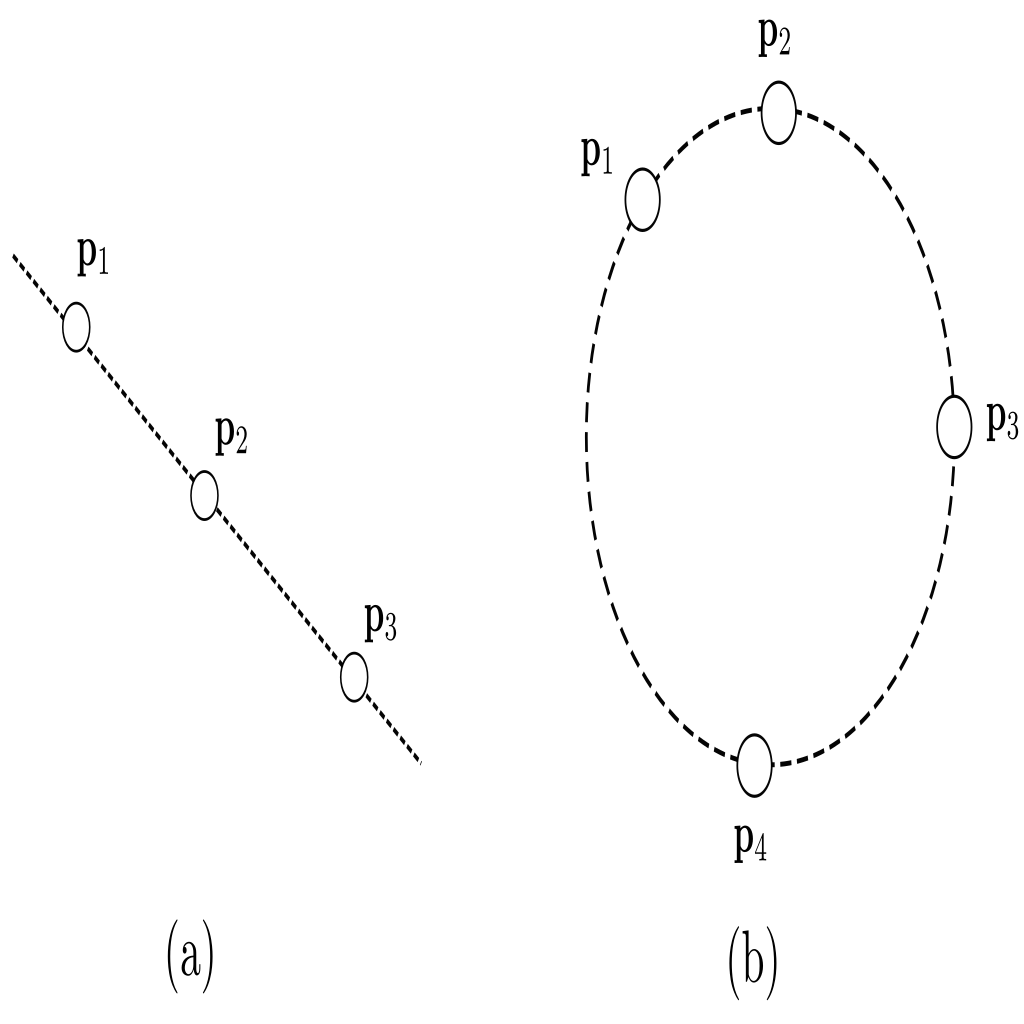
\includegraphics[width = 0.6\textwidth]{Chapter 2/17. not generic.png}
        \caption{(a) Three collinear nodes. (b) Four nodes arranged such that they lie on a circle.}
        \label{fig: not generic points}
    \end{figure}

\noindent
In Figure \ref{fig: not generic points} (a), we have three nodes $\mathbf{p}_1, \mathbf{p}_2, \mathbf{p}_3$ that are collinear. These points satisfy the equation $y = mx + c$, where $m \neq 0$, and $ m,c \in \mathbb{Q}$. As the nodes satisfy a non-zero polynomial with rational coefficients, this configuration of nodes is not generic. Similarly, the nodes $\mathbf{p}_1, \mathbf{p}_2, \mathbf{p}_3, \mathbf{p}_4$ in Figure \ref{fig: not generic points} (b) satisfies the equation $(x-a)^2 + (y-b)^2 = r^2$, where $r \neq 0$, and $a,b,r \in \mathbb{Q}$. Therefore, this configuration is not generic either.
\end{example}


\begin{flushleft}
Our definition of infinitesimal rigidity only apply to configurations that are generic as if we allow for non-generic configurations, things go awry. This is demonstrated when considering the infinitesimal motions of the framework $(G,\mathbf{p})$ in Figure \ref{fig: non-generic}.
\end{flushleft}

\begin{figure}[htbp]
    \centering
    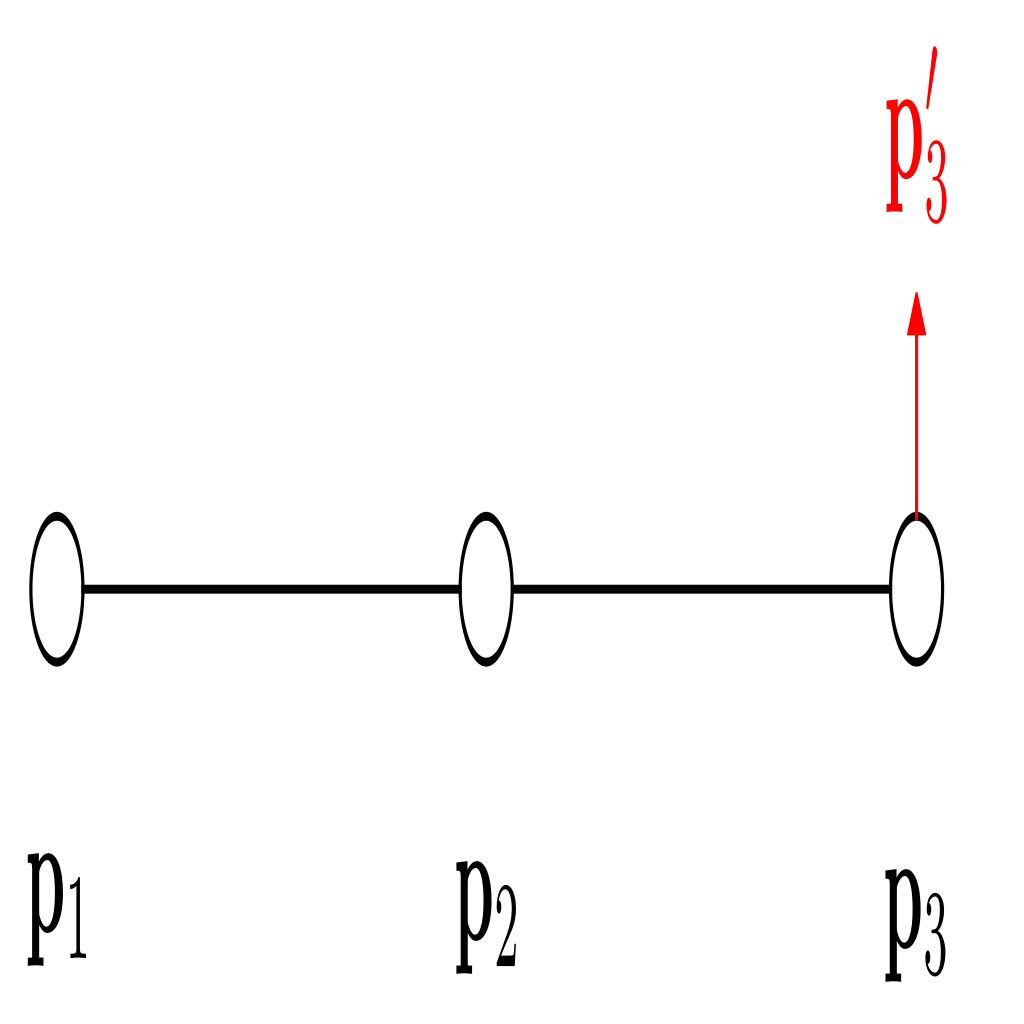
\includegraphics[width = 0.4\textwidth]{Chapter 2/16. generically_rigid.png}
    \caption{A non-generic framework in $\mathbb{R}^2$ with a non-zero instantaneous velocity applied to $\mathbf{p}_3$.}
    \label{fig: non-generic}
\end{figure}

\vspace{-2mm}
\begin{flushleft}
Here, the three nodes lie on a straight line and so they are not generic. Suppose we apply instantaneous velocities $\mathbf{p}'_1$, $\mathbf{p}'_2$ of magnitude 0 to the nodes $\mathbf{p}_1$ and $\mathbf{p}_2$ respectively, and apply the instantaneous velocity $\mathbf{p}'_3 = (0,k)$, where $k \in \mathbb{R}$, to the node $\mathbf{p}_3$.
\end{flushleft}

\begin{flushleft}
By observation, we can tell that this framework is not infinitesimally rigid. By fixing nodes $\mathbf{p}_1$ and $\mathbf{p}_2$ in space, we may rotate the edge $\mathbf{p}_2\mathbf{p}_3$ about $\mathbf{p}_2$, thereby changing the distance between the nodes $\mathbf{p}_1$ and $\mathbf{p}_3$. 
\end{flushleft}

\begin{flushleft}
By computing the scalar products stated in Definition \ref{def: inf motion}, we see that 
\end{flushleft}
\vspace{-0.5mm}
\[
(\mathbf{p}_1 - \mathbf{p_2}) \cdot (\mathbf{p}'_1 - \mathbf{p}'_2) = (\mathbf{p}_2 - \mathbf{p_3}) \cdot (\mathbf{p}'_2 - \mathbf{p}'_3) = 0
\]

\begin{flushleft}
for both edges $\mathbf{p}_1\mathbf{p}_2$ and $\mathbf{p}_2\mathbf{p}_3$. However, 
\end{flushleft}
\vspace{-0.5mm}
\[
(\mathbf{p}_1 - \mathbf{p_3}) \cdot (\mathbf{p}'_1 - \mathbf{p}'_3) = 0
\]

\begin{flushleft}
as $\mathbf{p}'_3$ is perpendicular to the line passing through $\mathbf{p}_1\mathbf{p}_3$, stating that this framework is infinitesimally rigid. 
\end{flushleft}

\begin{flushleft}
For this reason, the frameworks we concern ourselves with will be defined on generic coordinates. Finally, we conclude with what it means to be generically rigid.    
\end{flushleft}

\begin{theorem}
\label{thm: generic rigid}
\cite{textbook} Let $(G,\mathbf{p})$ be an infinitesimally rigid framework in $\mathbb{R}^d$. Then the framework $(G,\mathbf{q})$ is infinitesimally rigid for any generic configuration $\mathbf{q}$.
\end{theorem}

\begin{flushleft}
This is an extremely powerful result. If we can find a configuration $\mathbf{p} = (\textbf{p}_1, \hdots, \textbf{p}_n)$, such that $(G,\mathbf{p})$ is infinitesimally rigid, then Theorem \ref{thm: generic rigid} implies that for \textit{any} generic configuration $\mathbf{q} = (\textbf{q}_1, \hdots, \textbf{q}_n)$, we can find a framework with the same underlying graph $G$, such that it is also infinitesimally rigid.
\end{flushleft}

\begin{definition}
A framework $(G,\mathbf{p})$ is \textit{generically rigid} in $\mathbb{R}^d$ if it is infinitesimally rigid for any one configuration $\mathbf{p}$.
\end{definition}

\begin{flushleft}
With that, we conclude this introductory exploration into the definitions of rigidity. These concepts form the basis of everything that is to come in later chapters. 
\end{flushleft}

\begin{flushleft}
Our current objective is unravelling the multitude of theorems that surround the study of rigid frameworks. Through collecting as many tools revolving around rigidity and circle packings as possible and by invoking these ideas, we will be ever closer to understanding the structure of the special case of packings this project focuses on.
\end{flushleft}